\subsection{Completed six-benchmark run and analysis population}
\label{sec:qwen-corr-audit}

The Qwen numerical results use the run completed on September 17, 2026,
under \path{results/correlation_pipeline/reasoning-vllm-v1}. Forward replay
and the saved aggregate analyses are complete for 4,647 attempts from 1,547 source
problems: 500 MATH-500, 960 AIME24, 960 AIME25, 675 OlympiadBench, 1,280 AMC23,
and 272 Minerva attempts. AIME and AMC retain 32 attempts per problem;
the other benchmarks retain one. GPQA-Diamond and MMLU-Pro are absent.

This supersedes the September 15 tagged snapshot in the numerical report.
That historical snapshot had 738 inputs and 699 attempts after termination
filtering. The new run changes the population, termination policy, and token
scope together: it is not a controlled before/after comparison or an
annotation-only ablation. Historical snapshot outputs remain archived.

\paragraph{Generation, replay, and annotation.}
Generation serves \texttt{Qwen/Qwen3.5-35B-A3B-GPTQ-Int4} through vLLM with
temperature 0.6 and top-$p$ 0.95. Replay uses
\texttt{unsloth/Qwen3.5-35B-A3B} with runtime 4-bit quantization at the
probe-selected decoder indices 27, 34, 35, 36, 38, and 39.
Hidden-state features describe block inputs, not exact post-attention router
inputs. Router confidence is $1-H(p)/\log 256$. The continuation analysis
has 83 scalar features; across-layer means are emphasized and layerwise
screens remain exploratory. Saved bootstrap intervals use 500 replicates
and seed 42, resampling whole source problems.

The sentence judge is \texttt{unsloth/Qwen3.8-27B-NVFP4}, temperature zero,
thinking enabled with low reasoning effort, and a 4,096-token completion
budget. Inputs contain the question and previous/current/next sentences.
The frozen program SHA-256 is\par\noindent
\path{69706a02c0484f345cf57775729ce7551feb5932954b9ad0b8f5bb63585c6fd9}.
Its accuracy on these generated math traces has not been independently
measured; the earlier GGUF alignment evaluation uses a different deployment.

\paragraph{Population and token scopes.}
All supplied generations enter whole-continuation, full-reasoning, position,
and expert analyses, including token-limit completions. Whole-continuation
metrics include final-answer tokens. The \texttt{full/reasoning} view now
uses every reasoning token, independently of annotation coverage. Position
views also use all reasoning tokens within their absolute windows. Class
views alone use available validated sentence labels: the sampling protocol
selects sample zero, with error-rate-weighted benchmark quotas, seed 42,
and a 100,000-sentence cap. Missing labels never exclude a generation from
the other views. Missing class/window features are pairwise missing, not zero.

% Generated by generate_correlation_tables.py; numerical cells must not be edited.
\begingroup\scriptsize\setlength{\tabcolsep}{4pt}
\begin{longtable}{@{}lrrrrrrr@{}}
\caption{Completed-run coverage and accuracy, Qwen3.5-35B-A3B. All supplied attempts are retained, including limit hits. AIME/AMC use 32 attempts per problem; other benchmarks use one. Unparseable answers with known gold are incorrect. Pooled accuracy is descriptive.}\label{tab:qwen-corr-data}\\
\toprule
Dataset & Input & Limit hits & Analyzed & Correct & Errors & Input acc. & Analyzed acc. \\
\midrule\endfirsthead
\multicolumn{8}{l}{\textit{Continued from previous page}}\\
\toprule
Dataset & Input & Limit hits & Analyzed & Correct & Errors & Input acc. & Analyzed acc. \\
\midrule\endhead
\bottomrule\endfoot
MATH-500 & 500 & 17 & 500 & 345 & 155 & 0.690 & 0.690 \\
AIME24 & 960 & 105 & 960 & 817 & 143 & 0.851 & 0.851 \\
AIME25 & 960 & 165 & 960 & 773 & 187 & 0.805 & 0.805 \\
Olympiad & 675 & 89 & 675 & 322 & 353 & 0.477 & 0.477 \\
AMC23 & 1280 & 17 & 1280 & 1238 & 42 & 0.967 & 0.967 \\
Minerva & 272 & 19 & 272 & 73 & 199 & 0.268 & 0.268 \\
Pooled & 4647 & 412 & 4647 & 3568 & 1079 & 0.768 & 0.768 \\
\end{longtable}\endgroup

\begingroup\scriptsize\setlength{\tabcolsep}{4pt}
\begin{longtable}{@{}lrrrrrr@{}}
\caption{Whole-continuation aggregate features versus correctness: point-biserial $r$ (finite traces), Qwen3.5-35B-A3B. Token-limit completions are included. A dash denotes an undefined coefficient.}\label{tab:qwen-corr-correct}\\
\toprule
Feature & MATH-500 & AIME24 & AIME25 & Olympiad & AMC23 & Minerva \\
\midrule\endfirsthead
\multicolumn{7}{l}{\textit{Continued from previous page}}\\
\toprule
Feature & MATH-500 & AIME24 & AIME25 & Olympiad & AMC23 & Minerva \\
\midrule\endhead
\bottomrule\endfoot
Token count & $-0.291$ (500) & $-0.726$ (960) & $-0.727$ (960) & $-0.387$ (675) & $-0.238$ (1,280) & $-0.293$ (272) \\
Router confidence & $0.199$ (500) & $0.533$ (960) & $0.493$ (960) & $0.243$ (675) & $0.175$ (1,280) & $0.112$ (272) \\
Leading-expert margin & $0.125$ (500) & $0.562$ (960) & $0.479$ (960) & $0.218$ (675) & $0.295$ (1,280) & $0.075$ (272) \\
Selected probability mass & $0.131$ (500) & $0.175$ (960) & $0.342$ (960) & $0.188$ (675) & $0.097$ (1,280) & $0.082$ (272) \\
Selection-boundary margin & $0.054$ (500) & $-0.035$ (960) & $0.222$ (960) & $0.118$ (675) & $-0.010$ (1,280) & $0.039$ (272) \\
Selected/rest mean gap & $0.131$ (500) & $0.175$ (960) & $0.342$ (960) & $0.188$ (675) & $0.097$ (1,280) & $0.082$ (272) \\
Hidden-state norm & $0.203$ (500) & $-0.018$ (960) & $0.056$ (960) & $0.085$ (675) & $0.550$ (1,280) & $0.083$ (272) \\
Hidden-state step distance & $0.157$ (500) & $0.382$ (960) & $0.404$ (960) & $0.111$ (675) & $0.557$ (1,280) & $0.100$ (272) \\
Hidden/router geometry & $-0.152$ (500) & $-0.058$ (960) & $-0.077$ (960) & $-0.102$ (675) & $-0.229$ (1,280) & $-0.096$ (272) \\
Top-1 switch rate & $-0.071$ (500) & $-0.297$ (960) & $0.141$ (960) & $0.005$ (675) & $-0.160$ (1,280) & $-0.006$ (272) \\
Adjacent selected-set overlap & $0.047$ (500) & $0.022$ (960) & $-0.155$ (960) & $0.016$ (675) & $-0.062$ (1,280) & $-0.010$ (272) \\
\end{longtable}\endgroup


\paragraph{Termination and accuracy denominators.}
There are 3,568 correct answers among 4,647 attempts (0.768). All 412
completion-limit hits (8.9\%) remain in the analysis; only two are correct.
Among the 4,235 non-limited attempts, 3,566 are correct (0.842). There are
388 unparseable answers counted as incorrect under the known-gold scoring
contract. These denominators differ from accuracy computed only among
parseable answers in generation summaries. Termination and length are
strong potential confounders: these results do not estimate natural-length
performance or a length-adjusted routing effect.

\subsection{Correctness associations and uncertainty}

Whole-continuation router confidence has positive point-biserial coefficients
on all six benchmarks: MATH-500 $r=0.199$, AIME24 $0.533$, AIME25 $0.493$,
Olympiad $0.243$, AMC23 $0.175$, and Minerva $0.112$. Saved pointwise
95\% problem-bootstrap intervals exclude zero except for AMC23
($[-0.116,0.678]$). MATH-500's interval is $[0.099,0.276]$;
AIME24's is $[0.382,0.678]$ and AIME25's is $[0.302,0.608]$.
These are marginal associations, without length or dataset adjustment.

Leading-expert margin ($M=p_{(1)}-p_{(2)}$) is positive throughout; Minerva's interval includes
zero. Hidden-state step distance is also positive throughout
($r=0.100$--$0.557$), while token count is negative
($-0.727$--$-0.238$). The change from the historical snapshot's signs
cannot be attributed to adding labels alone: replay and inclusion semantics
also changed. Attempts within AIME/AMC problems are dependent; naive
trace-level $p$-values and their BH adjustments are diagnostic only.

\begin{figure}[p]
\centering
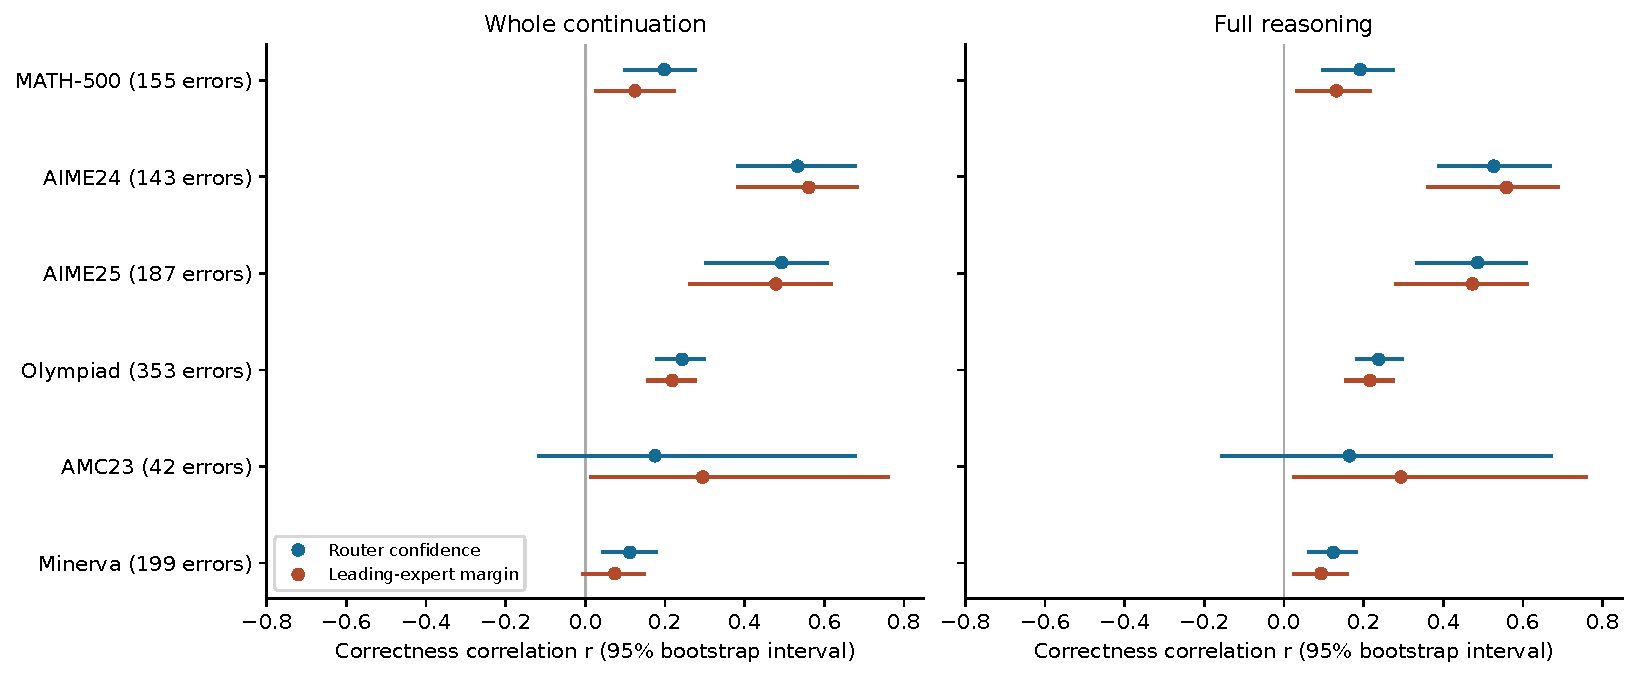
\includegraphics[width=\linewidth]{figures/qwen_correctness_intervals.pdf}
\caption{Qwen3.5 router confidence and leading-expert margin versus correctness,
with saved pointwise 95\% problem-bootstrap intervals across all six
benchmarks. Both views retain all attempts, including limit hits;
full reasoning excludes non-reasoning continuation tokens. Error counts
refer to attempts, not independent source problems.}
\label{fig:qwen-correctness}
\Description{Two panels show confidence and margin coefficients and intervals
for whole continuation and full reasoning across six benchmarks.}
\end{figure}

Full-reasoning confidence gives similar coefficients: $0.191$, $0.527$,
$0.486$, $0.238$, $0.164$, and $0.124$ in the same dataset order.
All 4,647 traces have reasoning tokens. Similarity between these two
scopes is descriptive; it does not remove length or termination effects.

\subsection{Class-conditioned routing and hidden states}
\label{sec:qwen-classes}

\begingroup\scriptsize\setlength{\tabcolsep}{4pt}
\begin{longtable}{@{}lrrrrrrrr@{}}
\caption{Class coverage in the completed run. Qwen3.8-27B labels on Qwen3.5-35B-A3B generations. Units are tagged sentences; dataset columns count traces with selected class tokens. Classes overlap across traces; missing classes are not zero-valued features.}\label{tab:qwen-class-coverage}\\
\toprule
Class & Units & MATH-500 & AIME24 & AIME25 & Olympiad & AMC23 & Minerva & Total traces \\
\midrule\endfirsthead
\multicolumn{9}{l}{\textit{Continued from previous page}}\\
\toprule
Class & Units & MATH-500 & AIME24 & AIME25 & Olympiad & AMC23 & Minerva & Total traces \\
\midrule\endhead
\bottomrule\endfoot
Read & 6,358 & 378 & 30 & 26 & 514 & 27 & 270 & 1245 \\
Analyze & 22,378 & 424 & 30 & 30 & 619 & 38 & 271 & 1412 \\
Plan & 5,654 & 407 & 28 & 28 & 507 & 28 & 271 & 1269 \\
Implement & 23,844 & 477 & 30 & 30 & 667 & 39 & 271 & 1514 \\
Explore & 7,151 & 260 & 28 & 27 & 474 & 22 & 251 & 1062 \\
Verify & 10,745 & 400 & 29 & 30 & 617 & 38 & 270 & 1384 \\
Monitor & 23,870 & 451 & 30 & 29 & 583 & 29 & 272 & 1394 \\
\end{longtable}\endgroup


The 100,000 sampled sentences have complete labels across 1,546 nonempty
attempt samples; one of the 1,547 sample-zero attempts has no labelled sentence.
All seven class analyses are complete, with coverage reported separately
from the full population. Explore has tokens in 1,062 traces; Verify in
1,384. AIME/AMC class views contain at most the 30/30/40 sample-zero
attempts rather than all 32 attempts per problem. Annotation counts describe
sampled sentences, not class prevalence in the complete corpus. Class
transition metrics require adjacent original tokens within the same sentence.

\begin{figure}[p]
\centering
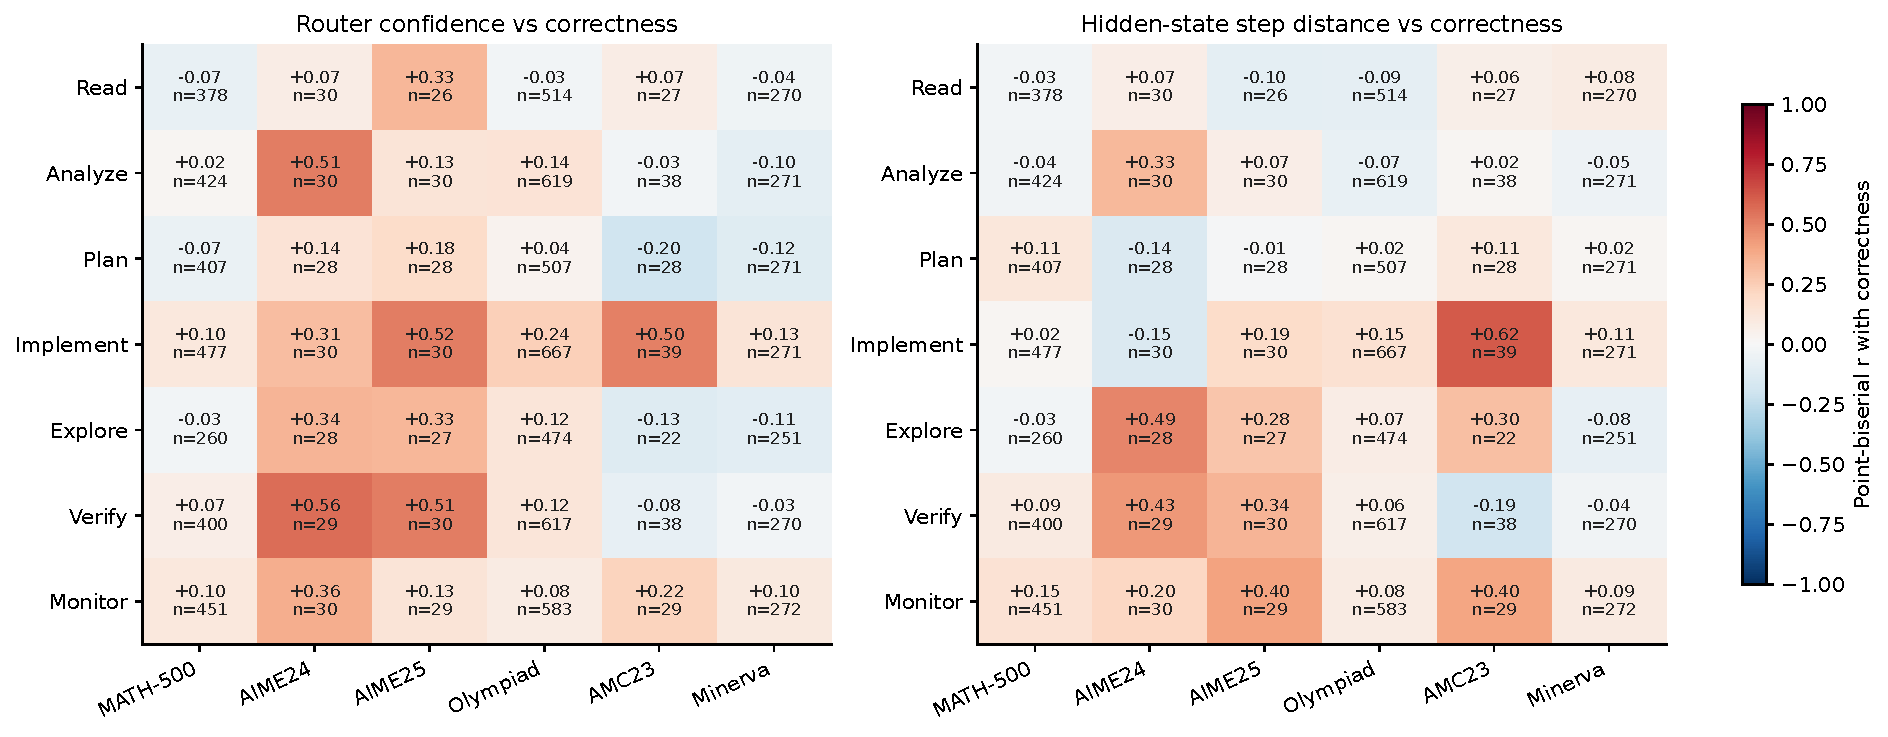
\includegraphics[width=\linewidth]{figures/qwen_class_correlations.pdf}
\caption{Class-conditioned confidence and hidden-state step distance versus
whole-attempt correctness. Cells show point-biserial $r$ and finite trace
count. Classes use sampled Qwen3.8 labels on Qwen3.5 generations, with
different token-bearing cohorts. No significance markings are implied.}
\label{fig:qwen-classes}
\Description{Two heatmaps compare seven predicted classes across six benchmarks,
with finite sample counts printed in each cell.}
\end{figure}

Class conditioning remains heterogeneous. Verify confidence is $0.066$
on MATH-500, $0.123$ on Olympiad, and $-0.028$ on Minerva; Plan confidence
is $-0.067$, $0.039$, and $-0.121$, respectively. These separately selected
cohorts do not test a difference between classes. The smaller AIME/AMC class
cohorts remain especially sensitive to individual errors. Annotation errors,
length, difficulty, and coverage are uncontrolled, so these screens do not
identify beneficial or harmful reasoning states.

\subsection{Class counts, transitions, and outcome associations}

The call distinguishes class-conditioned router features from the proportion
of reasoning assigned to each class (24:41--29:57). The following plots use
\emph{sampled sentence shares}: the number of labelled sentences of a class
divided by the number of labelled sentences in that attempt. An observed
zero share is retained; unlabelled sentences are never assigned a class.
These are estimates from the sampling protocol, not complete-sequence class
fractions. Each source problem contributes only its sample-zero attempt;
benchmark comparisons retain their separate denominators. Attempts with no
labelled sentences are excluded.

\begingroup\scriptsize\setlength{\tabcolsep}{4pt}
\begin{longtable}{@{}lrrrrrrrr@{}}
\caption{Mean sampled sentence share (percent), with equal weight per labelled attempt. Empty-label attempts are excluded; absent classes in an observed sample have zero share. These are not full-corpus class proportions.}\label{tab:class-shares}\\
\toprule
Dataset & Attempts & Read & Analyze & Plan & Implement & Explore & Verify & Monitor \\
\midrule\endfirsthead
\multicolumn{9}{l}{\textit{Continued from previous page}}\\
\toprule
Dataset & Attempts & Read & Analyze & Plan & Implement & Explore & Verify & Monitor \\
\midrule\endhead
\bottomrule\endfoot
MATH-500 & 499 & 8.9 & 19.5 & 9.3 & 29.3 & 4.1 & 11.8 & 17.1 \\
AIME24 & 30 & 6.7 & 33.9 & 2.9 & 28.3 & 7.0 & 14.4 & 6.8 \\
AIME25 & 30 & 5.7 & 33.2 & 4.8 & 27.9 & 6.7 & 13.4 & 8.3 \\
Olympiad & 675 & 6.9 & 26.8 & 6.0 & 29.7 & 6.4 & 13.2 & 11.0 \\
AMC23 & 40 & 6.6 & 25.9 & 5.8 & 32.0 & 3.8 & 15.2 & 10.6 \\
Minerva & 272 & 9.4 & 19.8 & 8.4 & 21.8 & 7.7 & 10.3 & 22.6 \\
\end{longtable}\endgroup


\begin{figure}[p]
\centering
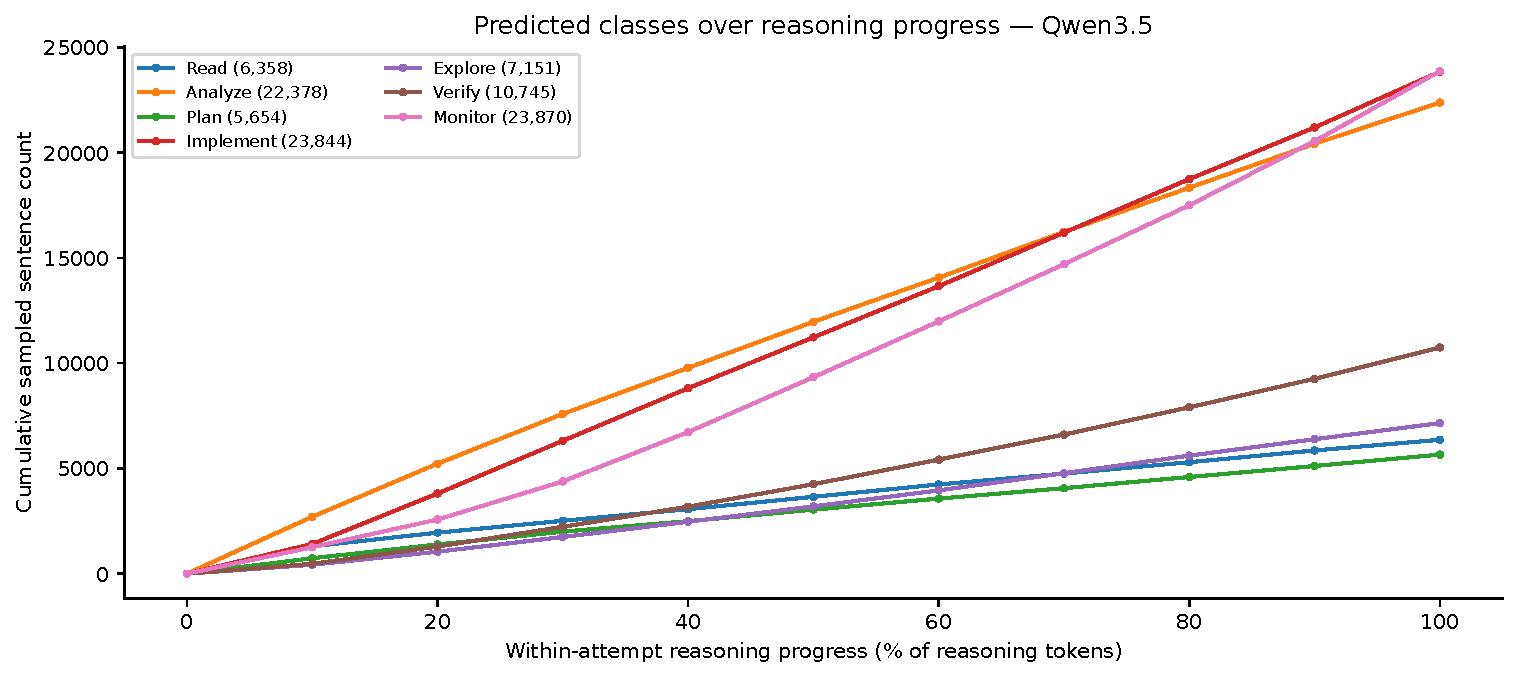
\includegraphics[width=\linewidth]{figures/qwen_class_cumulative.pdf}
\caption{Cumulative counts of sampled sentences by predicted class, pooled
across benchmarks. Counts start at zero; a sentence is counted when its last
reasoning token is reached. Progress is normalized by each attempt's full
reasoning-token length, unlike the absolute windows in
Figure~\ref{fig:qwen-position}. Legend totals equal the rightmost endpoints.
These are raw sampled counts, not cumulative percentages or estimates of
full-corpus counts; longer traces and benchmark sampling quotas affect them.}
\label{fig:class-cumulative}
\Description{Predicted sentence classes are summarized from sampled labels; the caption defines the counts, denominators, and outcomes.}
\end{figure}

\begin{figure}[p]
\centering
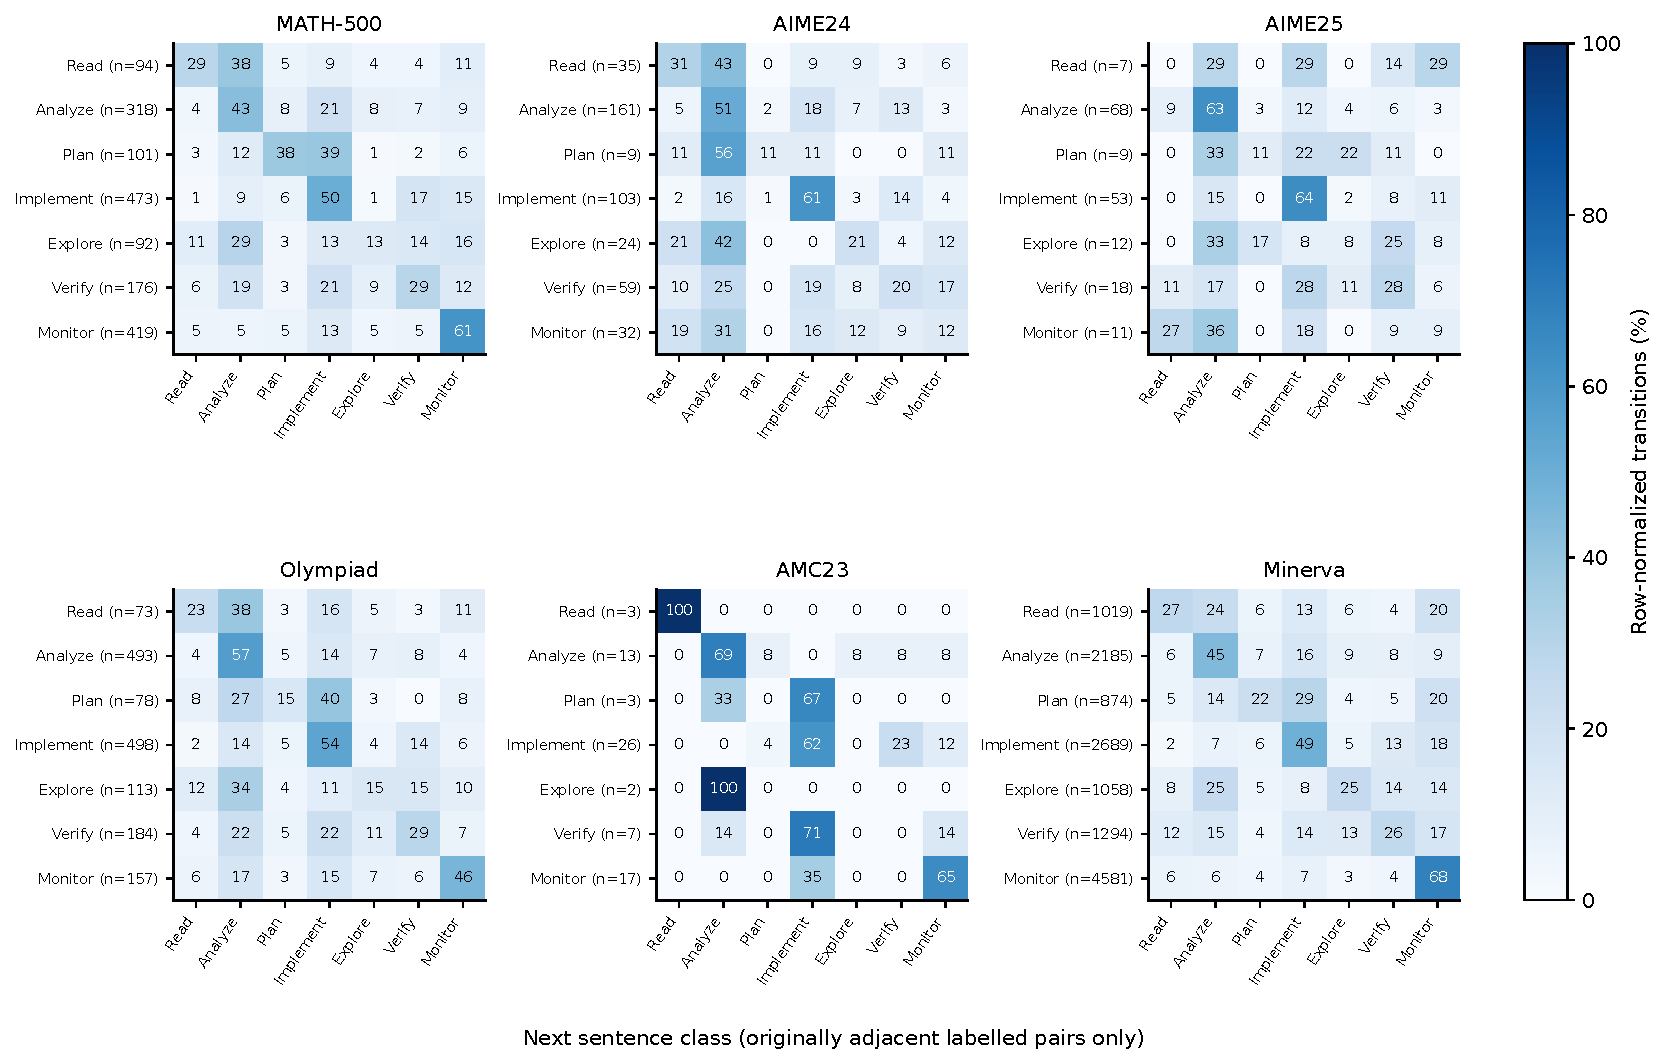
\includegraphics[width=\linewidth]{figures/qwen_class_transitions.pdf}
\caption{Observed class-state transitions by benchmark. Rows are the current
class, columns the next class; cells are row percentages and row labels give
pair counts. Only originally consecutive sentence indices with both labels
are counted. Gaps in sampling are never bridged. Self-transitions are retained;
empty rows are undefined. This describes the observed adjacent-pair sample,
not the complete transition process or an effect of changing state.}
\label{fig:class-transitions}
\Description{Predicted sentence classes are summarized from sampled labels; the caption defines the counts, denominators, and outcomes.}
\end{figure}

\begin{figure}[p]
\centering
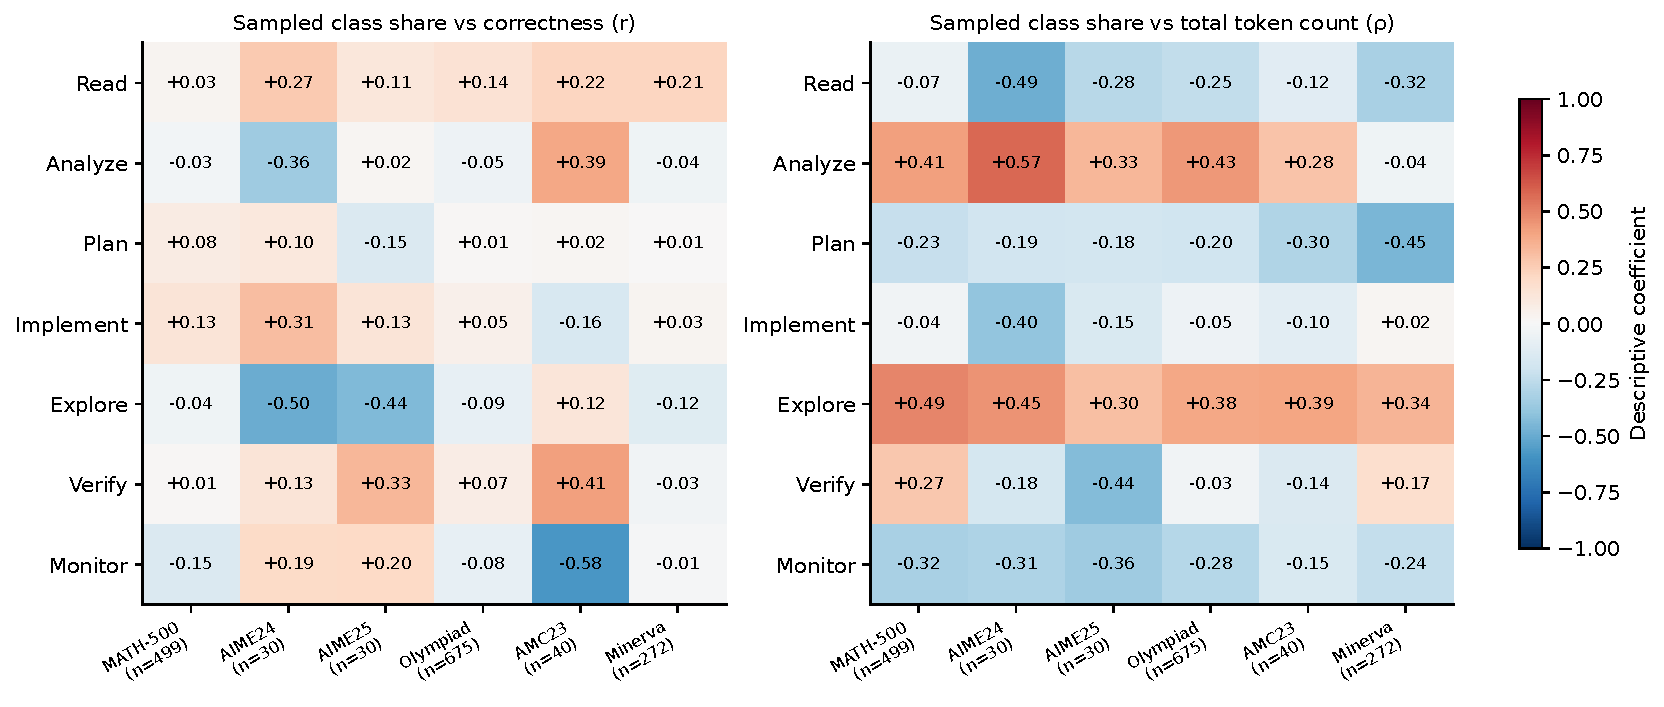
\includegraphics[width=\linewidth]{figures/qwen_class_share_correlations.pdf}
\caption{Sampled class proportions versus whole-attempt correctness
(point-biserial $r$) and total continuation-token count (Spearman $\rho$).
All labelled attempts enter each class, including observed zero proportions.
These differ from correlations of router features within class-selected
tokens. No significance claim is made; class shares sum to one and cannot
be interpreted as independent effects.}
\label{fig:class-share-correlations}
\Description{Predicted sentence classes are summarized from sampled labels; the caption defines the counts, denominators, and outcomes.}
\end{figure}

\begin{figure}[p]
\centering
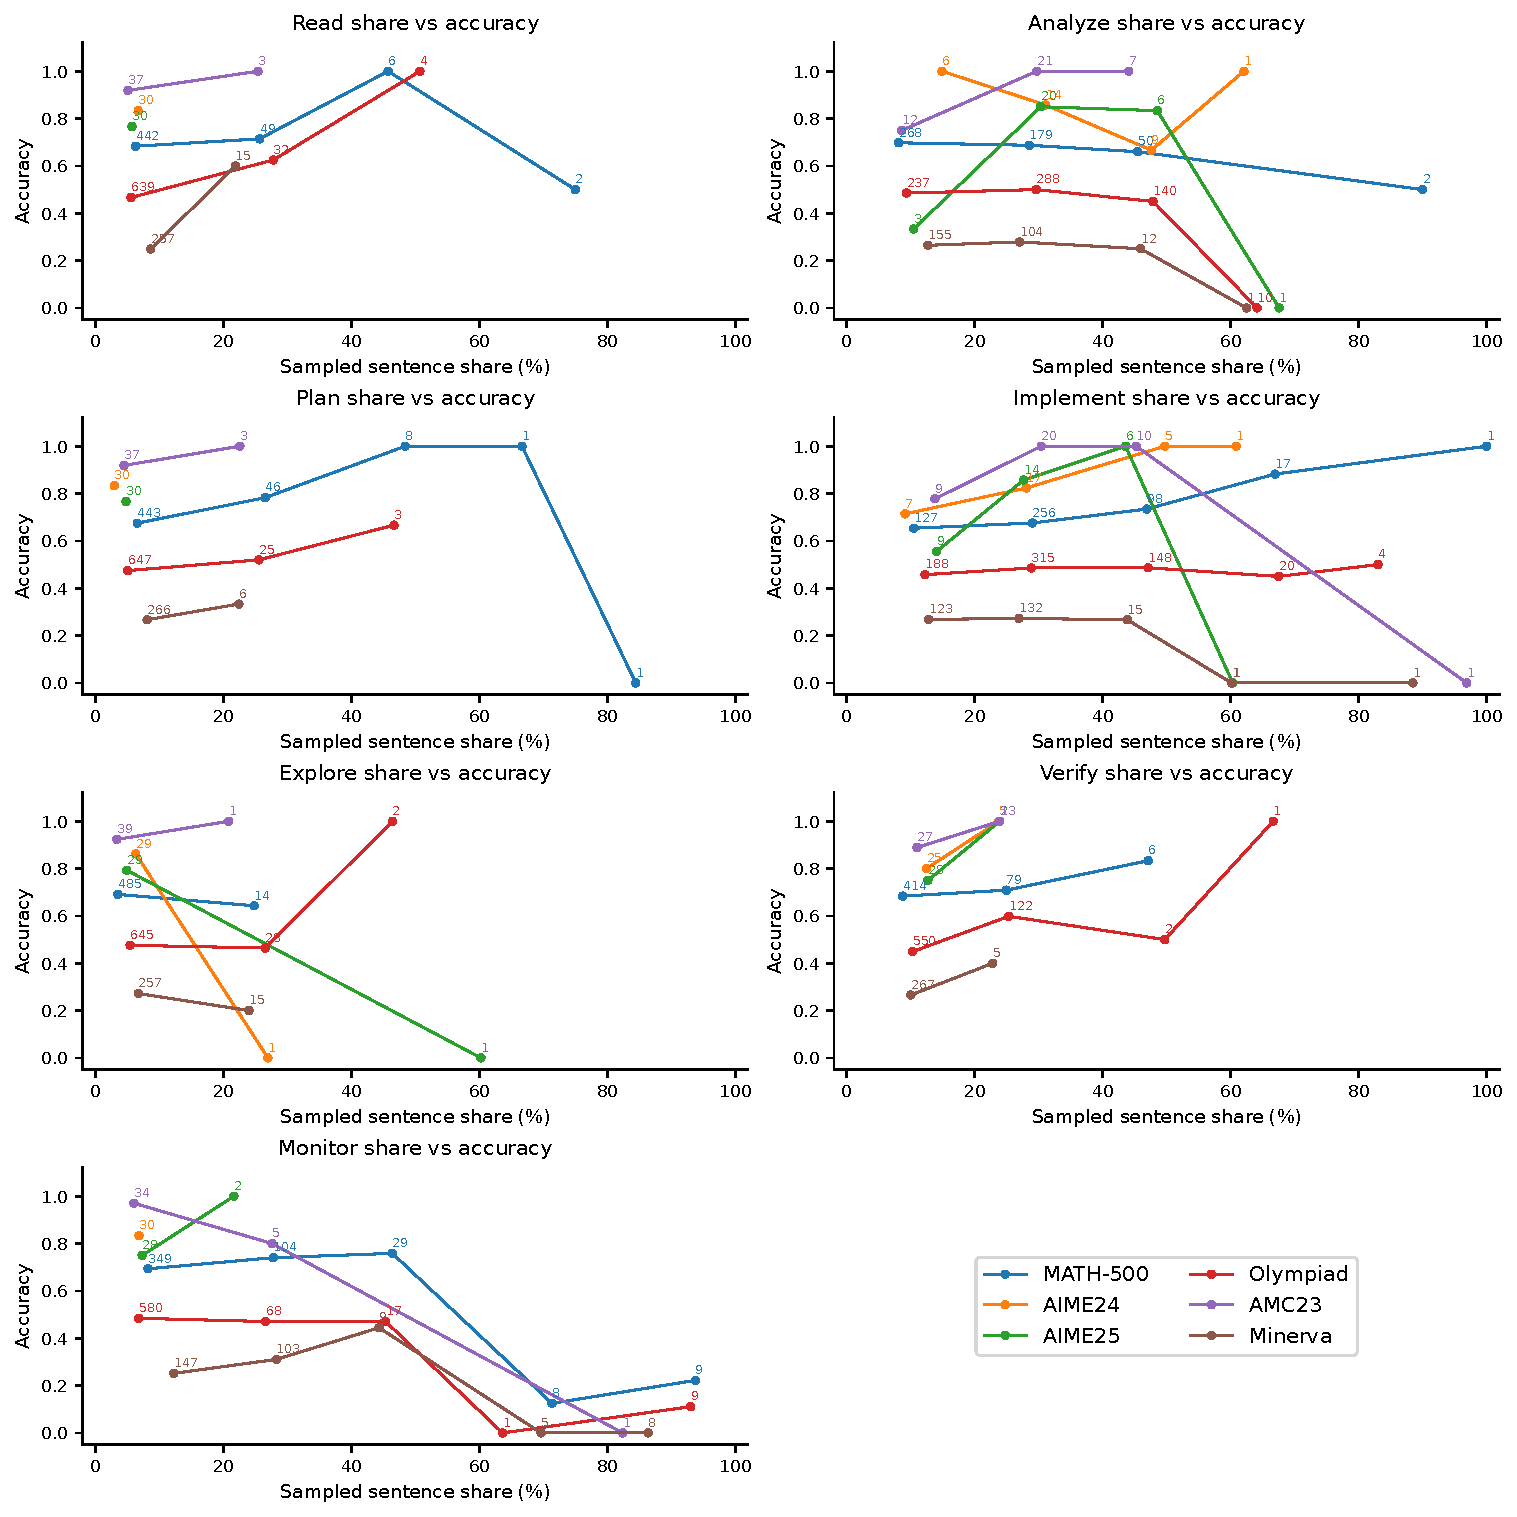
\includegraphics[width=\linewidth]{figures/qwen_class_share_accuracy.pdf}
\caption{Actual outcome levels versus sampled class proportions. Fixed share
bins are $[0,20)$, $[20,40)$, $[40,60)$, $[60,80)$, and $[80,100]$ percent.
Each point is at the mean observed share and shows accuracy; small labels give attempt counts. Empty
bins are omitted. Colours distinguish benchmarks; lines only connect
occupied bins. Sparse bins, sentence sampling, length, and difficulty can
explain apparent trends; these descriptive plots do not identify optimal
class proportions or a validated accuracy--length Pareto frontier.}
\label{fig:class-share-outcomes}
\Description{Predicted sentence classes are summarized from sampled labels; the caption defines the counts, denominators, and outcomes.}
\end{figure}

\begin{figure}[p]
\centering
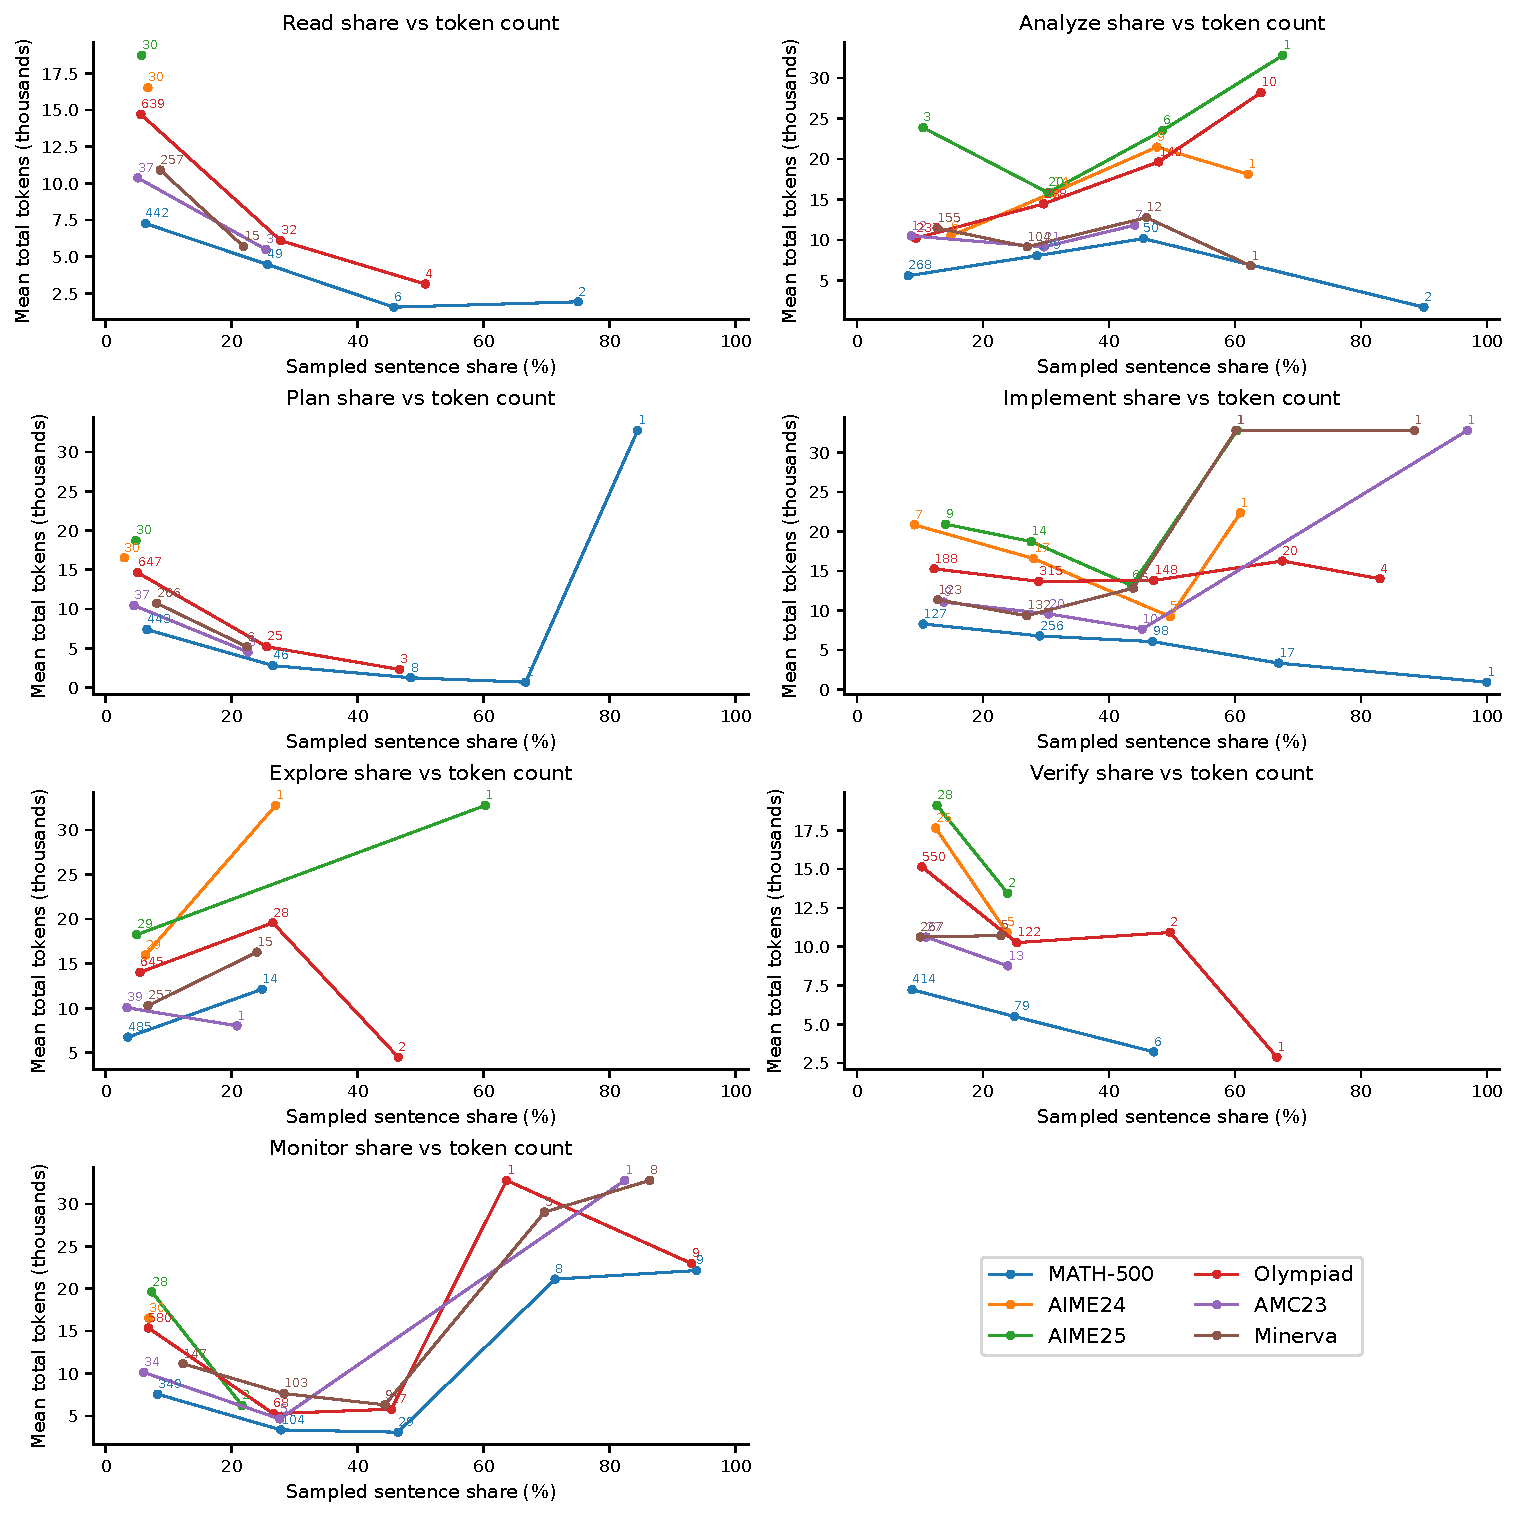
\includegraphics[width=.95\linewidth]{figures/qwen_class_share_tokens.pdf}
\caption{Mean total continuation tokens versus sampled class share. Bin
boundaries, colours, sample-count labels, and sampling limitations are as in
Figure~\ref{fig:class-share-outcomes}. Token count includes the final answer
and token-limit completions; lines are descriptive, not intervention effects.}
\label{fig:class-share-tokens}
\Description{Predicted sentence classes are summarized from sampled labels; the caption defines the counts, denominators, and outcomes.}
\end{figure}

Class-state dynamics remain descriptive. Relating complete transition paths
to correctness and interventions conditioned on those paths is future work,
as agreed at 29:32--30:20 and 45:23--48:10. The currently sampled labels do
not justify reconstructing missing transitions.


\subsection{Position-dependent estimates and coverage}

The position reference uses all 4,647 supplied generations and mean
reasoning length 12,498.062 tokens. Ten non-cumulative windows have boundaries
$\lceil i\bar{L}/10\rceil$, approximately 1,249.8 tokens apart; overflow
begins after the final boundary at 12,499. Every reasoning token contributes
to its window regardless of tagging. Token count is omitted as a position
predictor. Coverage falls from 4,647 traces in the first window to 1,789 in
overflow, so later-window coefficients describe different cohorts.

\begingroup\scriptsize\setlength{\tabcolsep}{4pt}
\begin{longtable}{@{}lrrrr@{}}
\caption{Reasoning length in tokens, all attempts including limit hits. This replaces the position-coverage count plot; lengths are observed under the generation budget.}\label{tab:reasoning-length}\\
\toprule
Dataset & Attempts & Mean & Median & 90th percentile \\
\midrule\endfirsthead
\multicolumn{5}{l}{\textit{Continued from previous page}}\\
\toprule
Dataset & Attempts & Mean & Median & 90th percentile \\
\midrule\endhead
\bottomrule\endfoot
MATH-500 & 500 & 6,226.5 & 4,250 & 12,772 \\
AIME24 & 960 & 15,908.4 & 14,011 & 32,766 \\
AIME25 & 960 & 17,874.9 & 16,620 & 32,768 \\
Olympiad & 675 & 13,402.5 & 9,150 & 32,768 \\
AMC23 & 1280 & 8,452.8 & 7,822 & 14,929 \\
Minerva & 272 & 9,805.0 & 7,465 & 19,533 \\
\end{longtable}\endgroup


\begin{figure}[p]
\centering
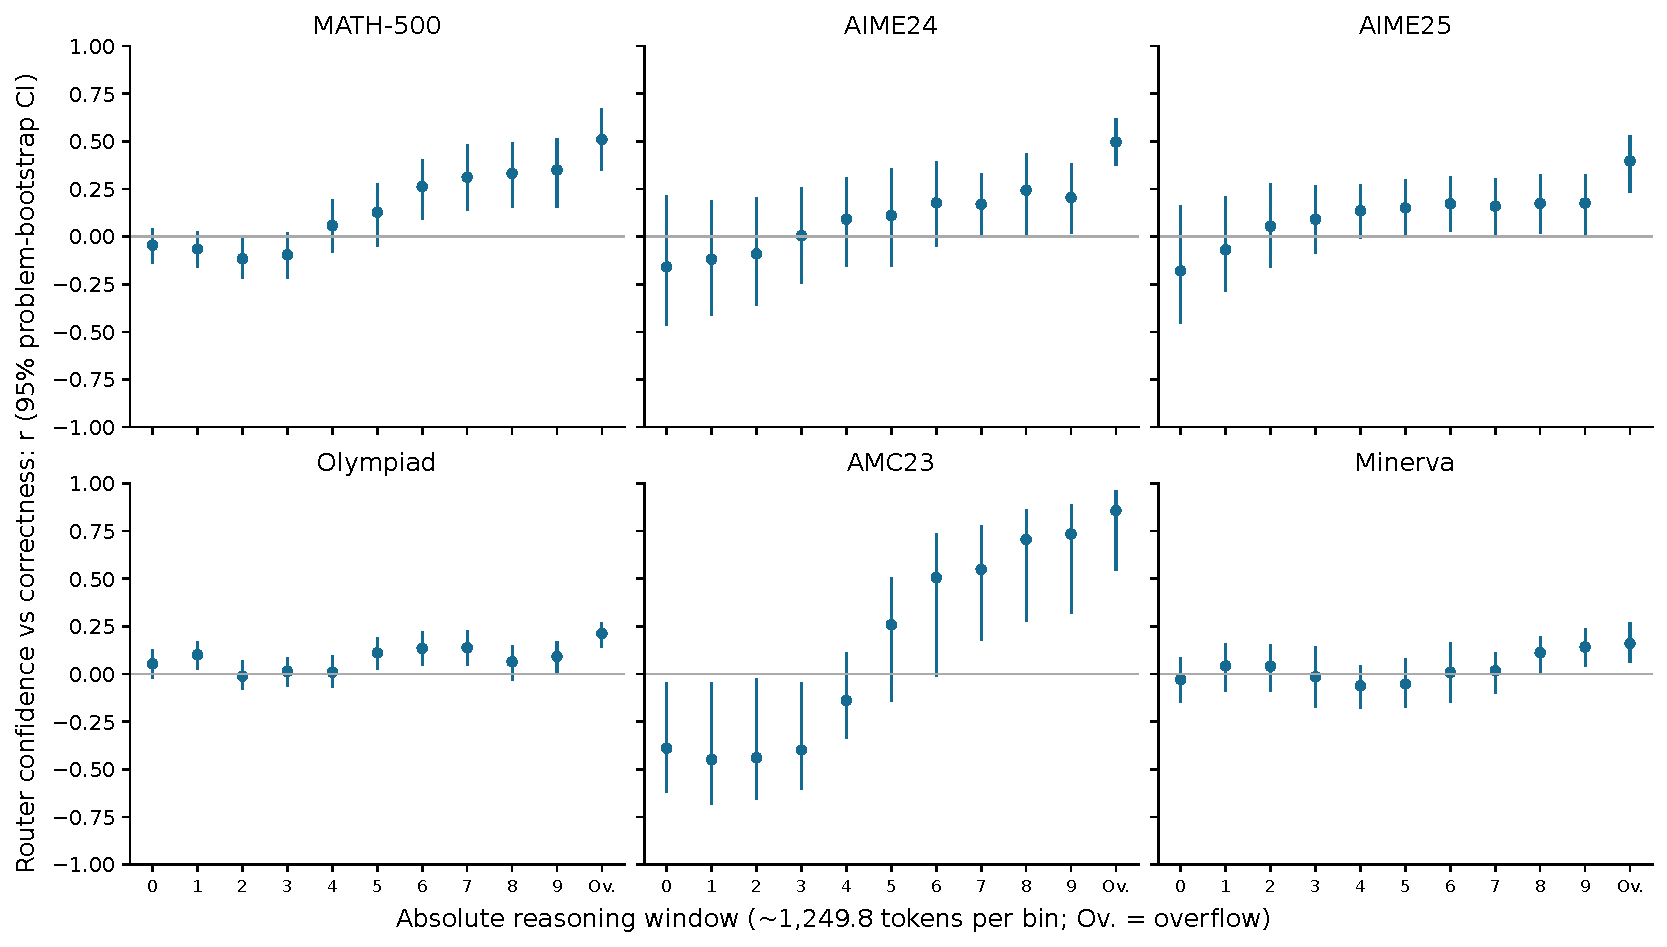
\includegraphics[width=\linewidth]{figures/qwen_position_coverage.pdf}
\caption{Router confidence versus whole-attempt correctness in absolute
reasoning windows, with saved pointwise 95\% source-problem bootstrap intervals.
Each benchmark has its own panel. Missing estimates remain blank. Later windows
use changing token-bearing cohorts; these are not within-trace causal effects.}
\label{fig:qwen-position}
\Description{Six panels show window-specific correlations and bootstrap intervals.}
\end{figure}

\subsection{Metric-pair dependence}

\begin{figure}[p]
\centering
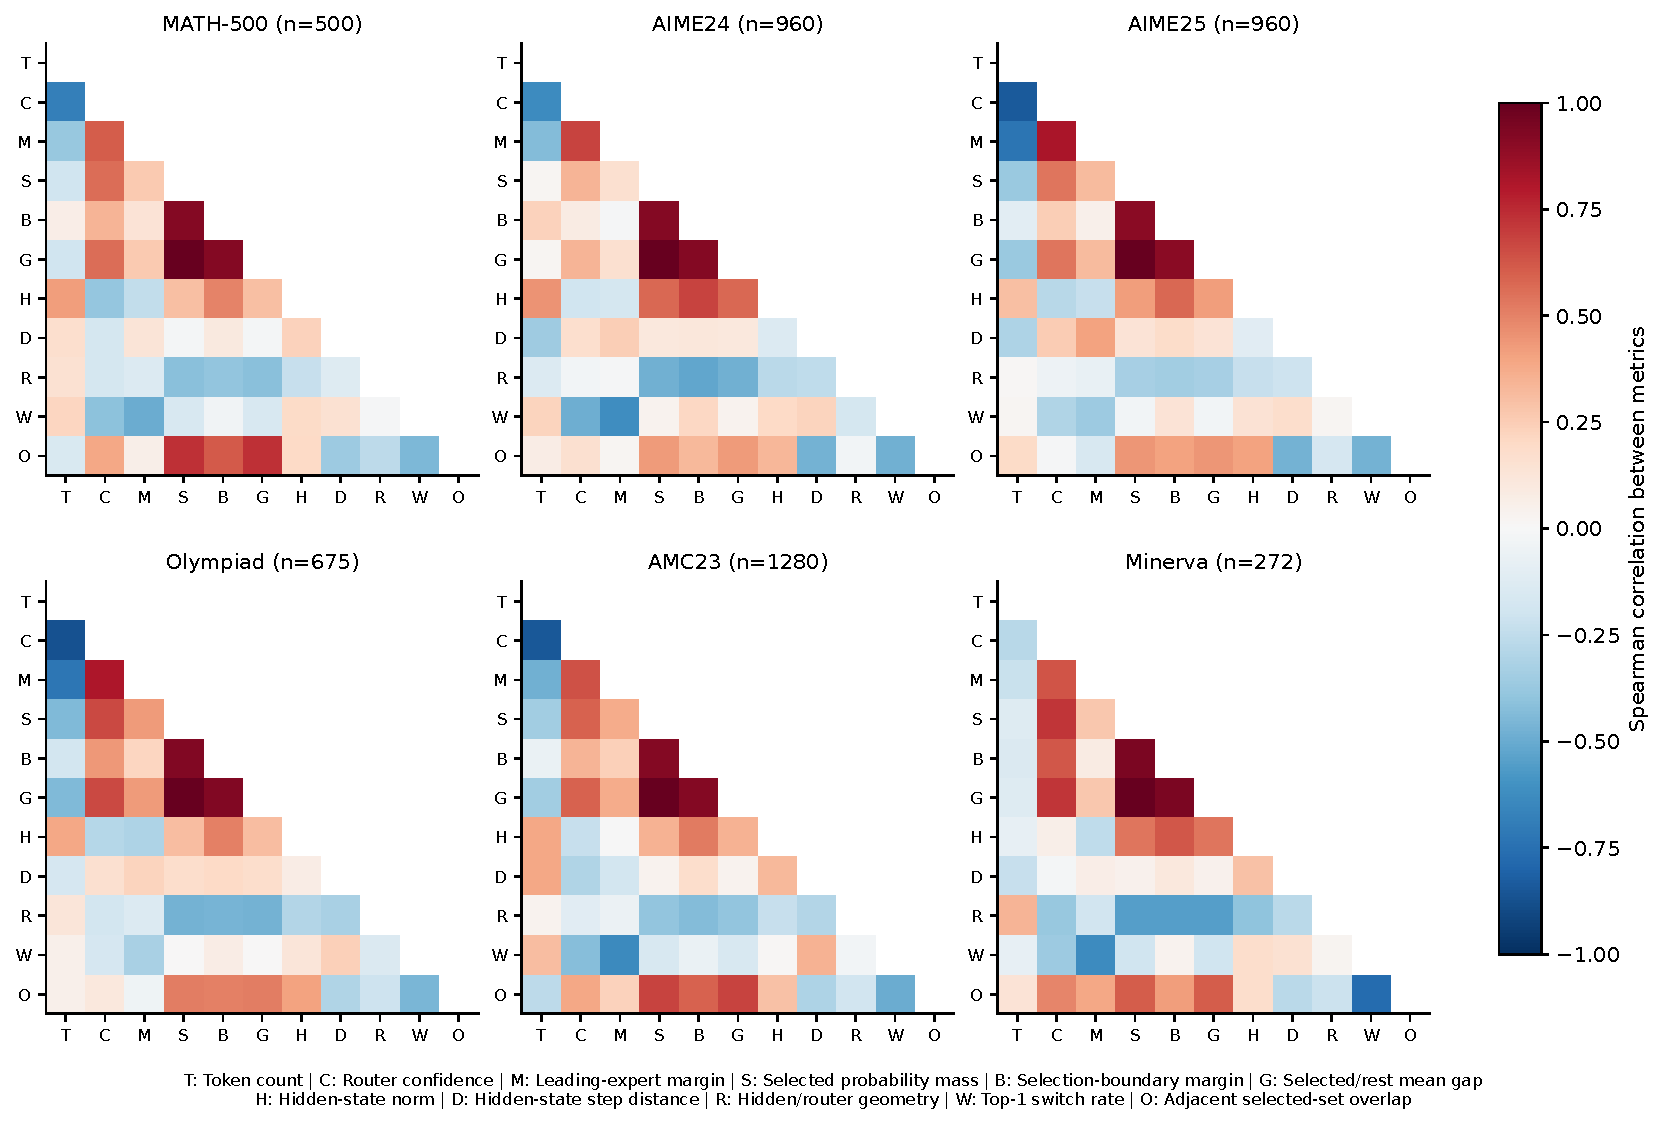
\includegraphics[width=\linewidth]{figures/qwen_metric_pairs.pdf}
\caption{Whole-continuation metric--metric Spearman correlations across all
six benchmarks. Lower triangles display each association once; diagonals
and upper triangles are omitted. Repeated attempts and limit hits remain
included. These are descriptive metric relationships, not correctness effects.}
\label{fig:qwen-metric-pairs}
\Description{Six triangular matrices compare eleven aggregate metrics, including
token count, confidence, margins, hidden-state features, and routing transitions.}
\end{figure}

Token count and confidence are negatively associated on all six datasets:
$\rho=-0.681$, $-0.627$, $-0.836$, $-0.870$, $-0.845$, and $-0.280$ in
MATH/AIME24/AIME25/Olympiad/AMC/Minerva order. This dependence is one reason
confidence--correctness correlations need length-aware follow-up.
Top-eight mass $S$ and the selected/unselected mean probability gap $G$
are algebraically redundant for $k=8$ and $E=256$:
\begin{equation}
G=\frac{S}{k}-\frac{1-S}{E-k}
 =\frac{E}{k(E-k)}S-\frac{1}{E-k}.
\end{equation}
The affine relation survives token/layer averaging. These metrics should
not count as independent corroboration or enter an unregularized model twice.
The appendix presents correlation heatmaps for all 20 scopes, including
class-conditioned metrics versus correctness and token count. The numeric
tables remain available as a separate generated artifact.

The legacy regex flags (backtracking, contradiction, and self-correction)
are removed from the report's outcome panels, as requested at 19:08--19:39.
They are not the seven predicted reasoning classes. Historical detector
outputs remain in the source artifacts.

\subsection{Repeated-attempt findings}

There are now 100 eligible complete avg@32 groups: 30 AIME24, 30 AIME25,
and 40 AMC23 problems. Problem means use all declared attempts, including
limit hits, and binary outcomes are complete. Unlike the historical
sample-zero snapshot, the current run supports both between-problem
rank associations and within-problem correct/incorrect contrasts.

\begingroup\scriptsize\setlength{\tabcolsep}{4pt}
\begin{longtable}{@{}lrrr@{}}
\caption{Whole-continuation mean feature versus avg@32 correctness, Spearman $\rho$ (source problems). All 32 attempts, including token-limit completions, enter each eligible group.}\label{tab:qwen-repeated}\\
\toprule
Feature & AIME24 & AIME25 & AMC23 \\
\midrule\endfirsthead
\multicolumn{4}{l}{\textit{Continued from previous page}}\\
\toprule
Feature & AIME24 & AIME25 & AMC23 \\
\midrule\endhead
\bottomrule\endfoot
Token count & $-0.861$ (30) & $-0.909$ (30) & $-0.057$ (40) \\
Router confidence & $0.632$ (30) & $0.705$ (30) & $-0.200$ (40) \\
Leading-expert margin & $0.583$ (30) & $0.638$ (30) & $0.190$ (40) \\
Selected probability mass & $-0.112$ (30) & $0.388$ (30) & $-0.215$ (40) \\
Selection-boundary margin & $-0.367$ (30) & $0.135$ (30) & $-0.145$ (40) \\
Selected/rest mean gap & $-0.112$ (30) & $0.388$ (30) & $-0.215$ (40) \\
Hidden-state norm & $-0.384$ (30) & $-0.186$ (30) & $0.484$ (40) \\
Hidden-state step distance & $0.238$ (30) & $0.384$ (30) & $0.504$ (40) \\
Hidden/router geometry & $0.273$ (30) & $0.046$ (30) & $-0.331$ (40) \\
Top-1 switch rate & $-0.381$ (30) & $0.156$ (30) & $0.121$ (40) \\
Adjacent selected-set overlap & $-0.047$ (30) & $-0.196$ (30) & $-0.327$ (40) \\
\end{longtable}\endgroup
\begingroup\scriptsize\setlength{\tabcolsep}{4pt}
\begin{longtable}{@{}lrrr@{}}
\caption{Within-problem confidence differences, Qwen3.5: mean correct minus incorrect, equally weighted over mixed-outcome problems; saved 95\% whole-problem bootstrap intervals.}\label{tab:qwen-within}\\
\toprule
Dataset & Mixed problems & Difference & 95\% interval \\
\midrule\endfirsthead
\multicolumn{4}{l}{\textit{Continued from previous page}}\\
\toprule
Dataset & Mixed problems & Difference & 95\% interval \\
\midrule\endhead
\bottomrule\endfoot
AIME24 & 14 & 0.00268 & [0.00152, 0.00412] \\
AIME25 & 15 & 0.00123 & [0.00065, 0.00176] \\
AMC23 & 6 & 0.01102 & [0.00455, 0.01709] \\
\end{longtable}\endgroup


Mean whole-continuation confidence correlates positively with avg@32 on
AIME24 ($\rho=0.632$, CI $[0.383,0.818]$) and AIME25
($0.705$, CI $[0.460,0.854]$). AMC23 is negative but uncertain
($-0.200$, CI $[-0.565,0.243]$), despite its positive attempt-level
coefficient. Thus attempt-level and problem-level associations answer
different questions. AIME24 and AIME25 mean token count have strong
negative avg@32 associations ($-0.861$ and $-0.909$).

\begin{figure}[p]
\centering
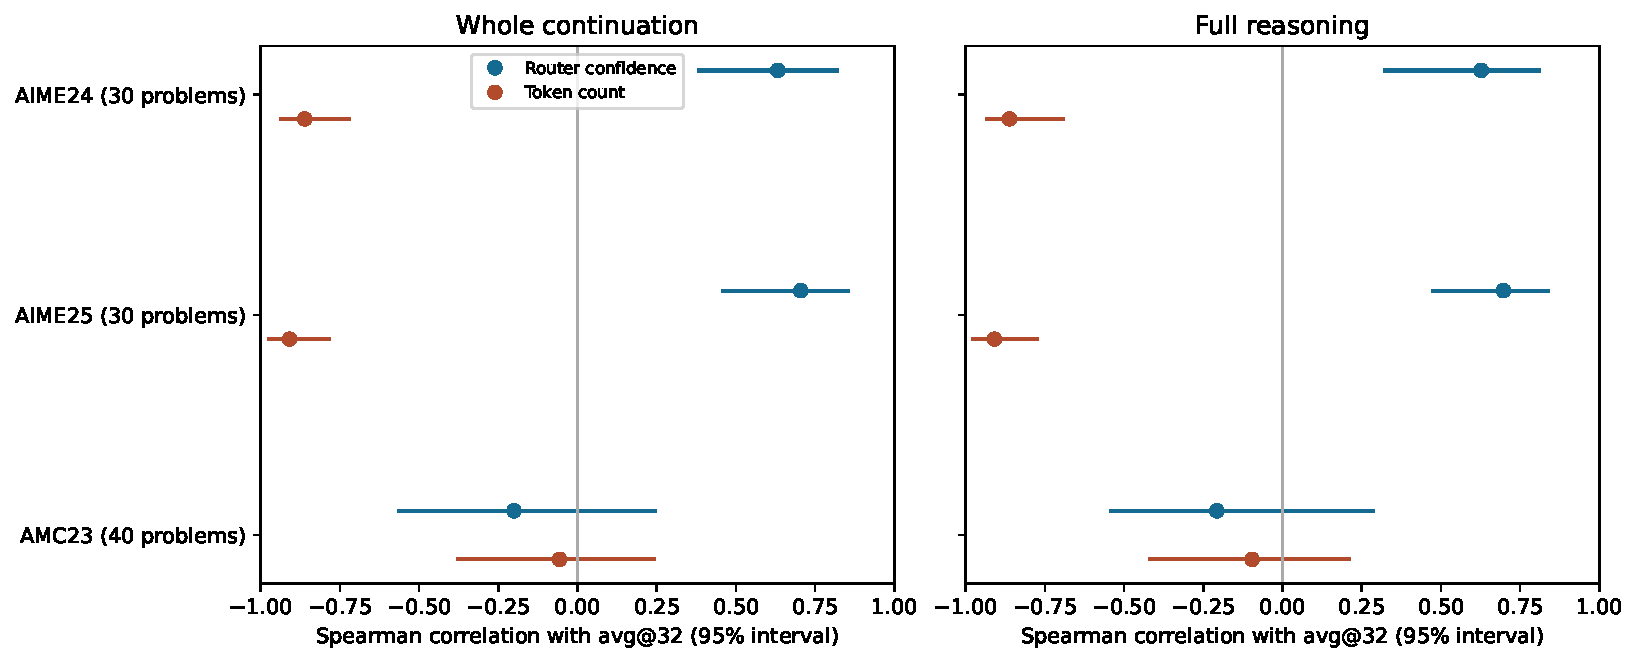
\includegraphics[width=\linewidth]{figures/qwen_repeated_intervals.pdf}
\caption{Mean confidence and token count versus problem-level avg@32,
with saved 95\% whole-problem bootstrap intervals. Whole-continuation and
full-reasoning views use the same complete 30/30/40 problem groups.
These estimates remain unadjusted for difficulty, length, and termination.}
\label{fig:qwen-repeated}
\Description{Two panels compare problem-level confidence and length rank
associations with avg@32 across AIME24, AIME25, and AMC23.}
\end{figure}

Within-problem confidence differences are positive over 14, 15, and 6
mixed-outcome problems, respectively; Table~\ref{tab:qwen-within} reports
magnitudes and bootstrap intervals. Conditioning on a shared question
reduces between-question variation but does not control attempt length or
termination. Class views still lack repeated labelled attempts, so these
repeated-attempt findings must not be generalized to class-specific effects.

\subsection{Expert screen, storage, and implications}

\begingroup\scriptsize\setlength{\tabcolsep}{4pt}
\begin{longtable}{@{}llrrrr@{}}
\caption{Post-hoc largest absolute correctness coefficient per dataset in the expert-rate screen, Qwen3.5-35B-A3B. Point-biserial $r$ and BH $q$ within dataset/target; no expert bootstrap intervals. Numeric IDs pool six distinct layer-local modules. Repeated-attempt trace-level q-values are diagnostic, not cluster-adjusted inference.}\label{tab:qwen-corr-experts}\\
\toprule
Dataset & Pooled-ID rate & Traces & Errors & $r$ & $q$ \\
\midrule\endfirsthead
\multicolumn{6}{l}{\textit{Continued from previous page}}\\
\toprule
Dataset & Pooled-ID rate & Traces & Errors & $r$ & $q$ \\
\midrule\endhead
\bottomrule\endfoot
MATH-500 & Top-1 61 / top-2 7 & 500 & 155 & $0.328$ & $3.36e-11$ \\
AIME24 & Top-1 ID 123 & 960 & 143 & $-0.568$ & $1.87e-80$ \\
AIME25 & Top-1 133 / top-2 85 & 960 & 187 & $0.556$ & $4.72e-76$ \\
Olympiad & Top-1 70 / top-2 181 & 675 & 353 & $0.312$ & $6.25e-14$ \\
AMC23 & Top-8 ID 217 & 1280 & 42 & $-0.665$ & $2.83e-161$ \\
Minerva & Top-1 162 / top-2 165 & 272 & 199 & $0.409$ & $1.31e-09$ \\
\end{longtable}\endgroup


The expert screen includes top-1 rates, any-top-eight rates, and up to 128
ordered top-1/top-2 pairs selected by routing support (minimum four traces).
The largest absolute correctness coefficient per dataset is selected
post hoc. Figure~\ref{fig:expert-outcomes} shows all selected-pool IDs against
correctness and total token count, without selecting a maximum. Numeric IDs pool six different layer-local modules; they do not
identify a portable expert or establish an intervention target. Trace-level
BH values on repeated-attempt datasets do not account for clustering.

\begin{figure}[p]
\centering
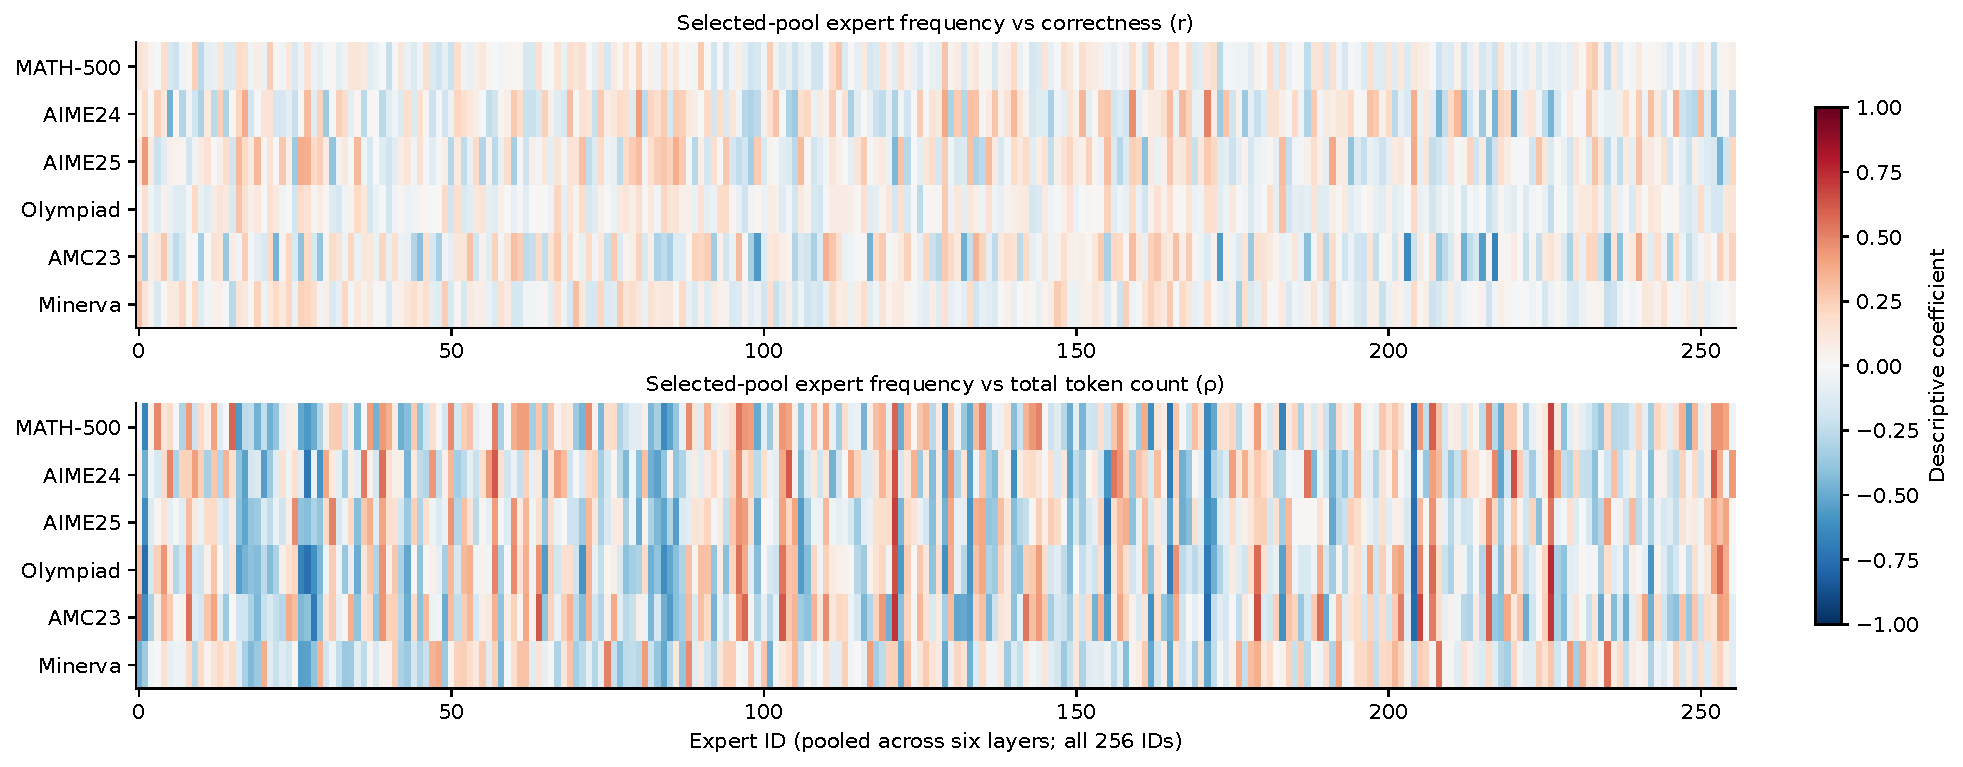
\includegraphics[width=\linewidth]{figures/qwen_expert_outcomes.pdf}
\caption{Selected-pool membership frequency for every expert ID versus
correctness ($r$, top) and total continuation tokens ($\rho$, bottom).
All 256 IDs are shown in their original order for each benchmark. Rates
pool tokens and six layers; the same ID refers to distinct layer-local
modules. These associations do not establish that activating an expert
will improve accuracy or reduce length.}
\label{fig:expert-outcomes}
\Description{Router features are compared with whole-attempt outcomes across six benchmarks; the caption defines the estimates and uncertainty.}
\end{figure}

\paragraph{Metric values associated with accuracy.}
Correlation signs alone do not specify the observed metric ranges associated
with higher accuracy (42:06--45:17). Figure~\ref{fig:router-value-accuracy}
therefore reports accuracy directly against router confidence, the
selection-boundary margin, and the selected/rest mean probability gap.
Bins are computed separately per benchmark; this is an exploratory
whole-continuation analysis, not an online threshold-selection experiment.

\begin{figure}[p]
\centering
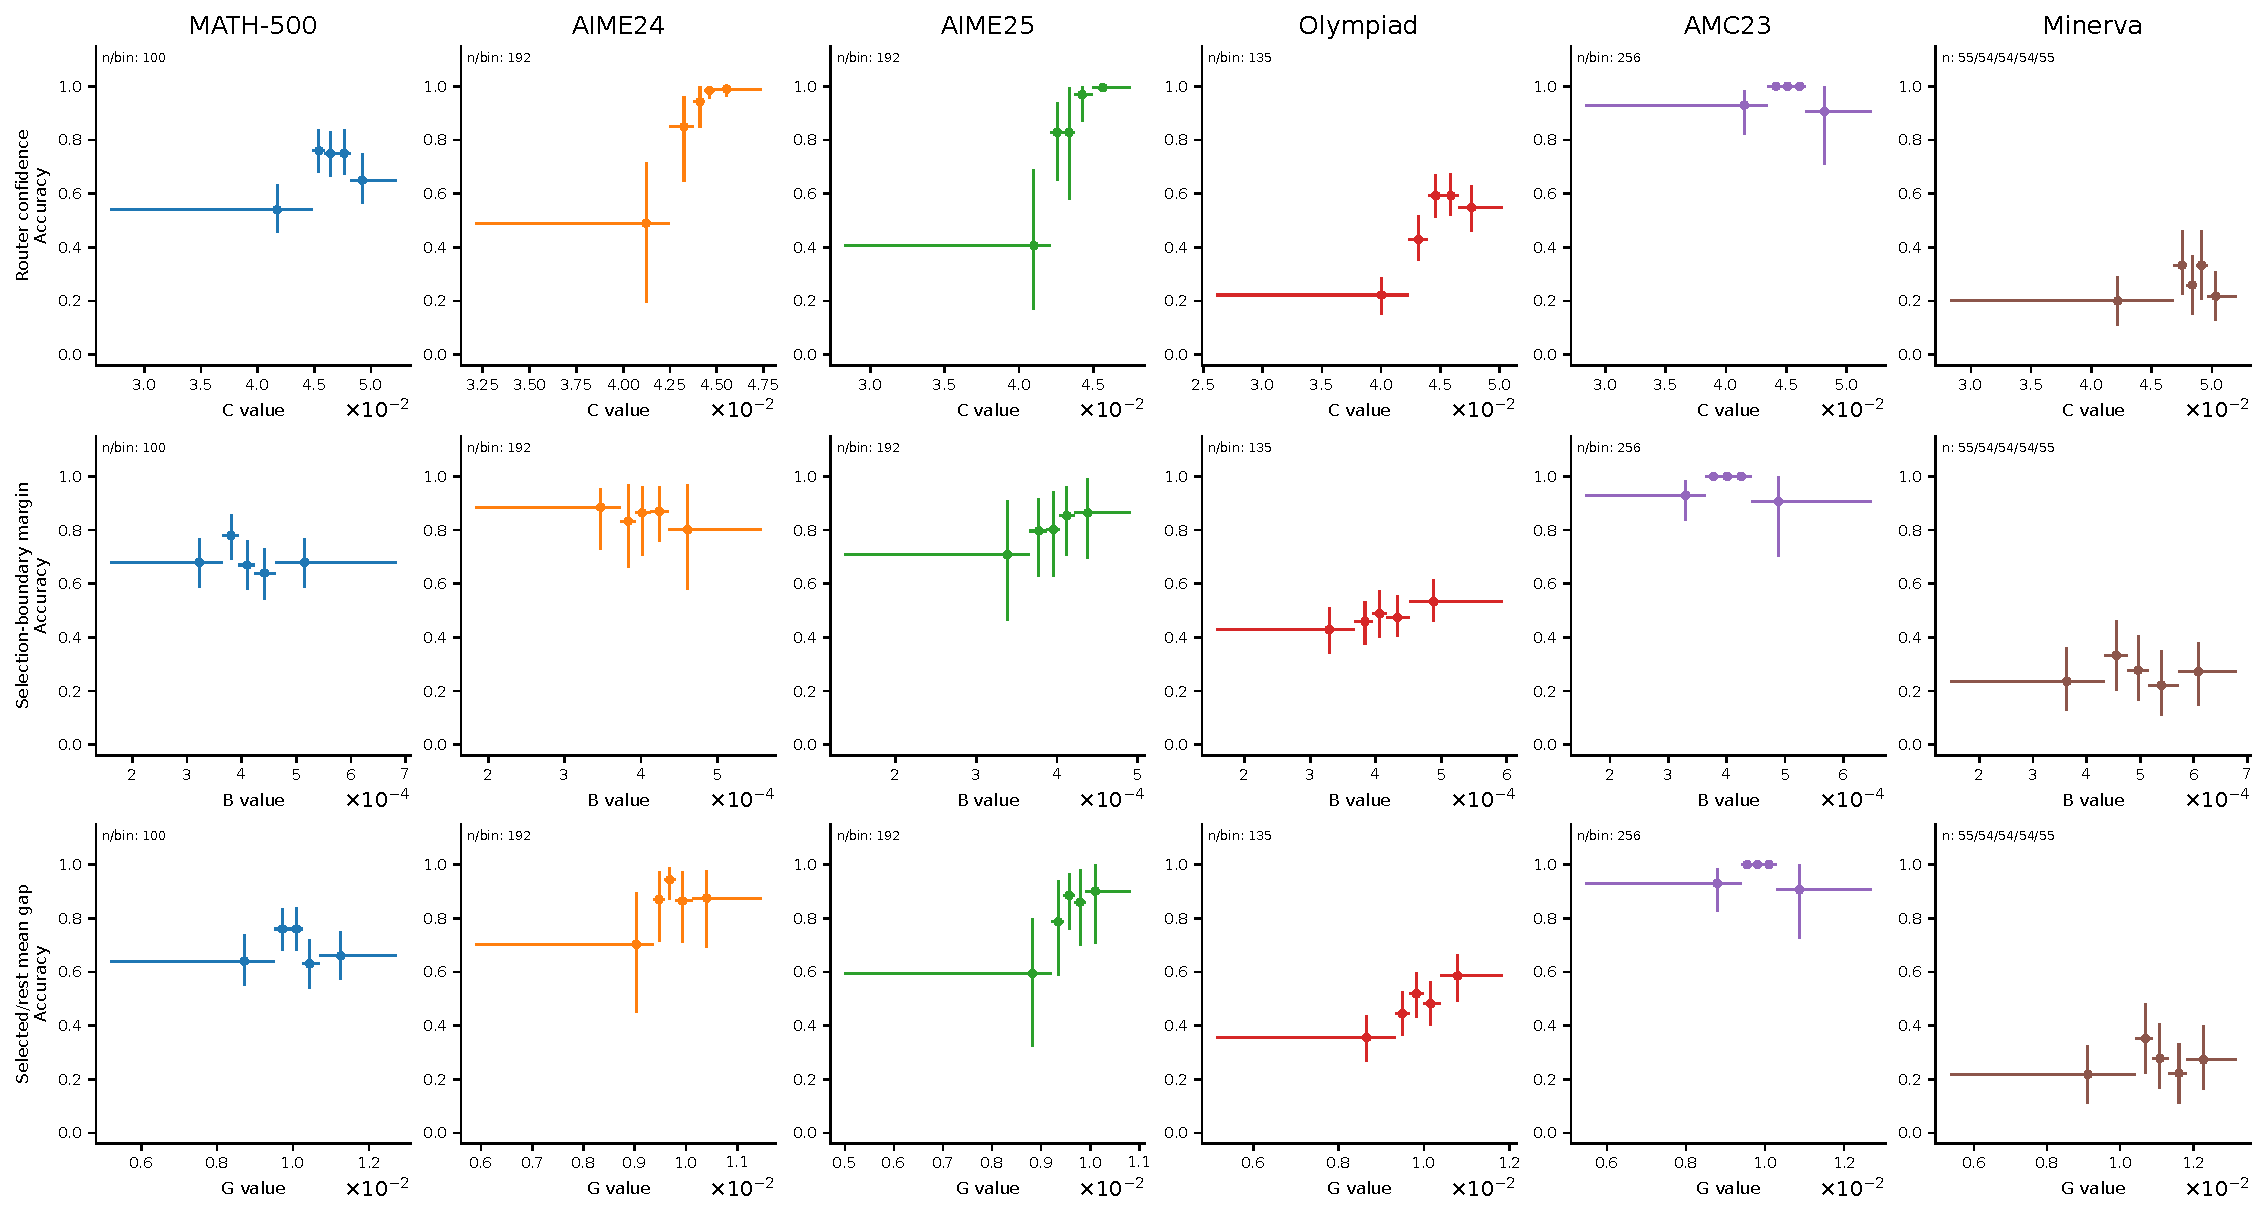
\includegraphics[width=\linewidth]{figures/qwen_router_value_accuracy.pdf}
\caption{Accuracy at observed router-metric values. Each benchmark uses
up to five quantile bins; horizontal bars show actual value ranges, points
show mean values and accuracy, and panel labels give attempt counts
per bin (left to right, or a shared count when equal). Vertical
bars are pointwise 95\% percentile intervals from 500 whole-source-problem
bootstrap resamples within each fixed bin (seed 42). Degenerate intervals
can occur in all-correct/all-incorrect bins and do not imply certainty.
All attempts and limit hits are retained. Bins can share source problems,
so their estimates are not independent; neither bin selection nor length
and termination confounding is addressed by these intervals.}
\label{fig:router-value-accuracy}
\Description{Router features are compared with whole-attempt outcomes across six benchmarks; the caption defines the estimates and uncertainty.}
\end{figure}

\paragraph{Common router notation and unavailable extensions.}
Let $p_{(j)}$ denote the $j$th largest router probability, $E$ the number
of experts, and $k$ the selected count ($E=256$, $k=8$ here). Router
confidence is $C=1-H(p)/\log E$; leading-expert margin is
$M=p_{(1)}-p_{(2)}$; selected probability mass is
$S=\sum_{j\leq k}p_{(j)}$; selection-boundary margin is
$B=p_{(k)}-p_{(k+1)}$; and selected/rest mean gap is
$G=S/k-(1-S)/(E-k)$. Thus $M$ is not a selected-versus-rest statistic.
These model-independent names replace ambiguous top-8/top-9 plot labels
without changing the saved metric definitions.

The requested rank-prefix curves (top 2, 4, 6, then all selected versus
the rest; 20:11--21:07 and 37:29--39:20) require additional probability
summaries. Only the all-selected endpoint $G$ is saved. Separate entropy
of the selected and unselected distributions also cannot be recovered
from global entropy, selected mass, or expert IDs. These extensions
require new feature extraction/replay; no missing curves are fabricated.


Replay covers 62,088,209 continuation tokens. Compact tensor artifacts
occupy 5.970 GB versus a projected 1,907.350 GB of raw selected-layer
payload; dataset files total 9.259 GB (decimal units).
Storage and source-fingerprint checks are recorded in
\path{report/correlation_run_audit.json}. No raw router/hidden tensors or
expert weights are saved. The completed run supplies six-benchmark,
full-reasoning, class, position, lexical, and repeated-attempt analyses.
Next steps are independent label assessment, length-/termination-aware
models, common-cohort class/window comparisons, and validation holding out
whole problems before any routing intervention.
